\documentclass[twoside]{article}
\usepackage[utf8]{inputenc}
\usepackage{lipsum}
\usepackage{breqn}
\usepackage{framed}
\usepackage{graphicx}
\usepackage{epsfig}

\usepackage{microtype} % Slightly tweak font spacing for aesthetics
\usepackage[hmarginratio=1:1,top=32mm,columnsep=20pt]{geometry} % Document margins
\usepackage{multicol} % Used for the two-column layout of the document
\usepackage{hyperref} % For hyperlinks in the PDF

\usepackage[hang, small,labelfont=bf,up,textfont=it,up]{caption} % Custom captions under/above floats in tables or figures
\usepackage{booktabs} % Horizontal rules in tables
\usepackage{float} % Required for tables and figures in the multi-column environment - they need to be placed in specific locations with the [H] (e.g. \begin{table}[H])

\usepackage{paralist} % Used for the compactitem environment which makes bullet points with less space between them

\usepackage{abstract} % Allows abstract customization
\renewcommand{\abstractnamefont}{\normalfont\bfseries} % Set the "Abstract" text to bold
\renewcommand{\abstracttextfont}{\normalfont\small\itshape} % Set the abstract itself to small italic text


\title{\vspace{-15mm}\fontsize{18pt}{4pt}\selectfont\textbf{Modeling of a Damped Triple Pendulum}} % Article title
\author{
\large
\textsc{Nick Eyre \& Jeff Holzgrafe}\\[2mm] % Your name
\normalsize Franklin W. Olin College of Engineering \\ % Your institution
\normalsize ENGR 2340: Dynamics \\ % Your institution
\normalsize \href{mailto:neyre@students.olin.edu,jeffrey.holzgrafe@students.olin.edu}{neyre@students.olin.edu, jeffrey.holzgrafe@students.olin.edu} % Your email address
\vspace{-5mm}
}
\date{}

\begin{document}

\maketitle

\begin{abstract}
    \noindent Compound triple pendulums are an obvious extension of the common choatic double pendulum problem. In this project, we model a planar compound triple pendulum both with and without viscous damping forces.  Using Lagrangian energy methods, we derive coupled ordinary differential equations of motion for the system and submit them to numerical integration in MATLAB to model the dynamics of the system. We use an experimental test setup with motion tracking  to collect experimental data for a compound triple pendulum which we compare to the simulated results.  After tuning the damping constants of the model to match those of the system, we acheived extremely close agreement between the model and the experimental results.  The inclusion of damping in the system significantly changes the dynamics, highlighting the system's chaotic nature.

\end{abstract}

\begin{multicols}{2} % Two-column layout throughout the main article text
    \section{Background}
The double pendulum is a classic system used in Dynamics courses everywhere.  Over the course of the class, we have solved equations of motion and simulated models of both simple (massless bars) and compound (bars with mass) planar double pendulums using Newton's Second Law and Euler's Equations.  In this project, we hope to extend the double pendulum system we have studied so well into a triple compound pendulum with damping at the joints.  The experimental system we are trying to model is shown in figure \ref{expsetup}.  The bars of the pendulum have significant mass, requiring the inclusion of rotational dynamics in the system. Furthermore, the system has been observed to damp significantly over time. To solve these equations of motion, we will explore the use of Lagrangian Mechanics for non-conservative systems and will solve for equations of motion.  We will create a numerical simulation for the system in order to explore our equations of motion and will validate them by comparison to experimental data from a real planar triple pendulum system. 

\begin{figure}[H]
\centering
\includegraphics[scale=0.3]{testsetup.JPG}
\caption{Experimental Test Setup.}
\label{expsetup}
\end{figure} 

The system in question is considerably more complicated than the traditional double pendulum studied. The bars of the pendulum have significant mass, that is, the pendulum is not a set of bobs joined by strings, but a set or bars with joints. Furthermore, the joints are not neccesarily frictionless. A picture of the experimental setup we hope to model is shown in Figure \ref{expsetup}.

The tools necessary to complete this modeling came almost entirely from Dynamics lectures.  Additional reading$^{1,4}$, however, was done on use of Lagrangian energy methods for nonconservative systems. Numerous sources$^{2,3}$ present a derivation of the equations of motion of a double pendulum using energy methods. However, we were unable to find any sources which derived the equations of motion of a triple pendulum. Several sources$^{5}$ show simulations of triple pendulums: we used these to validate our model.


    \section{Learning Objectives}
In our double pendulum simulation, we found that our model predicted the behavior of the experimental setup quite well for the first few seconds, but soon after diverged rapidly into a completely different path. We pointed to the lack of friction in our model as the likely cause of this error. Even though friction has a small effect, the chaotic nature of the double pendulum means that any small perturbation can vastly change the dynamics.

We wanted to further investigate this outstanding question for our final project. As we had previously analyzed a double pendulum using Newtonian methods, we chose to model a triple pendulum with energy methods in order to cover new material. While energy methods are useful only in a small subset of real-world dynamics problems, they are nonetheless an interesting and wildly different approach. Furthermore, we were interested in learning how to represent friction in a complex system, which we have done little in the class so far. 

Overall, for our project we are interested in studying how changes in damping parameters of a system change the dynamics. This will allow us to investigate our hypothesis that the chaotic behaviour of a muliple pendulum system causes wildly divergent behaviour with the introdcution of small friction forces.  Furthermore, we want to learn more about the use of energy methods with nonconservative systems.

    \section{Model}
The experimental setup we hope to model is shown in Figure \ref{expsetup}. The bars of the pendulum have significant mass so it is modeled as a compound pendulum. We will also include damping in the model in order to study its effects on the choatic behaviour of the system.

A schematic representation of the system is shown in Figure \ref{model}. Each bar $i$ is defined by a set of four parameters: $I_i$, the moment of inertia of the bar, $m_i$, the mass of the bar, $l_i$, the length of the bar, and $k_i$, the damping coefficient of the bar rotating about it's upper joint. The position and velocity of the bars are defined by the six system state variables: $\theta _1, \theta _2, \theta _3, \dot{\theta _1}, \dot{\theta _2},\dot{\theta _3}$. 

\begin{figure}[H]
\centering
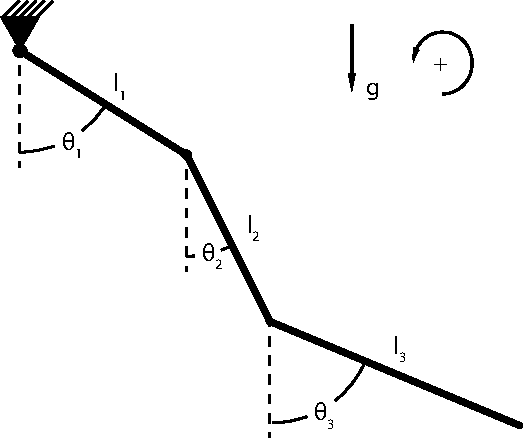
\includegraphics[scale=0.7]{Diagram.pdf}
\caption{Schematic representation of the model.}
\label{model}
\end{figure} 

We first derive the equations of motion of the frictionless ideal case. This allows for model validation by ensuring energy is conserved in the dynamics. Later we will add in frictional damping, and see how it changes the dynamics.

Taking down as +y and right as +x, we write the positions of the centers of mass of the bars as functions of $\theta _i$ and the geometric parameters of the system.

\begin{equation}
y_1 = \frac{l_1}{2}\cos \theta_1
\end{equation}
\begin{equation}
y_2 = l_1\cos \theta _1 + \frac{l_2}{2}\cos \theta_2
\end{equation}
\begin{equation}
y_3 = l_1\cos \theta _1 + l_2\cos \theta_2 + \frac{l_3}{2} \cos \theta _3
\end{equation}
\begin{equation}
x_1 = \frac{l_1}{2}\sin \theta_1
\end{equation}
\begin{equation}
x_2 = l_1\sin \theta _1 + \frac{l_2}{2}\sin \theta_2
\end{equation}
\begin{equation}
x_3 = l_1\sin \theta _1 + l_2\sin \theta_2 + \frac{l_3}{2} \sin \theta _3
\end{equation}

These positions are then differentiated with respect to time to find the x and y components of the velocities as functions of angles and angular velocities. They will not be shown here for brevity.

The magnitude of the velocity of each bar is
\begin{equation}
v_i = \sqrt{\dot{x_i}^2+\dot{y_i}^2}
\end{equation}
The translational and rotational kinetic energiy (TKE and RKE) of each bar is:
\begin{equation}
TKE_i = \frac{1}{2}m_iv_i^2
\end{equation}
\begin{equation}
RKE_i = \frac{1}{2}I_i\dot{\theta_i}
\end{equation}
The gravitational potential energy(GPE) of each bar is:
\begin{equation}
GPE_i = m_igy_i
\end{equation}

Using these, the Lagrangian of the system is:
\begin{equation}
\mathcal{L} = T-V = \displaystyle\sum_{i=1}^{3} TKE_i+RKE_i-GPE_i
\label{lagrangian}
\end{equation}

Equation \ref{lagrangian} can then be input to Lagrange's Equation:
\begin{equation}
\frac{d}{dt}(\frac{d\mathcal{L}}{\dot{q_i}})=\frac{d\mathcal{L}}{dq_i}
\end{equation}
where $\theta _i$ is used for the generalized coordinate $q_i$. This yields a system of three equations which contain the angular acceleration terms, omitted for brevity. The solution of this system of three equations and three unknowns yields the expressions for the angular velocities. We then numerically integrate these angular velocities to produce the path of the pendulum. A characteristic plot of the path is shown in Figure \ref{paths}. Energy is conserved in the undamped simulation, and the pendulum appears to behave as expected.  An animation of the system was also created and used to validate the results.  Videos of the animation are posted on YouTube for chaotic (\href{http://youtu.be/7lNIAdsInMg}{http://youtu.be/7lNIAdsInMg}) and periodic (\href{http://youtu.be/_THTgIZqDGQ}{http://youtu.be/_THTgIZqDGQ}) intial conditions.  With this validation of our basic methods, we add damping to the system. 

The bars of the experimental setup are thin, and the velocities are generally low, so we chose to model the system damping with a viscous drag caused by the angular velocity of the joints. This viscous form of drag can be modeled in Lagrangian mechanics with the Rayleigh Dissipation Function:
\begin{equation}
D = \frac{1}{2}(\displaystyle\sum_{i=1}^{3}k_i\dot{\theta _i}^2)
\end{equation}
Lagranges equation is the rewritten as
\begin{equation}
\frac{d}{dt}(\frac{d\mathcal{L}}{\dot{q_i}})=\frac{d\mathcal{L}}{dq_i}-\frac{dD}{d\dot{q_i}}
\end{equation}

This modified form of Lagrange's equation produces a system of three equations which contain the angular velocity terms, as above for the undamped case. Solving for the angular velocity terms produces the equations of motion shown in Appendix A.




    \section{Results}
After creating and validating or model, we collected exprimental data for a triple pendulum which had been constructed by Ben Smith for the course.  The parameters of this experimental test setup were measured (Table \ref{expparams}) and input into our simultaion.  The triple pendulum was tracked by an OptiTrack vision tracking system and the data was parsed with a Python script in order to return angles as functions of time for the three links.  This vision tracking was set up by professor Aaron Hoover.  Velocity data for the three links was created through numerical differentiation and a low-pass filter using MATLAB's filter function.

\begin{table}[H]
\centering
 \begin{tabular}{|l|l|l|}
        \hline
        Parameter & Value    & Unit        \\ \hline
        $m_1$     & 0.2944   & kg          \\ 
        $m_2$     & 0.1756   & kg          \\ 
        $m_3$     & 0.0947   & kg          \\ 
        $l_1$     & 0.508    & m           \\ 
        $l_2$     & 0.254    & m           \\ 
        $l_3$     & 0.127    & m           \\ 
        $I_1$     & 9.526e-3 & kg$\cdot$ m^2 \\ 
        $I_2$     & 1.625e-3 & kg$\cdot$ m^2 \\ 
        $I_3$     & 1.848e-4 & kg$\cdot$ m^2 \\ 
        $k_1$     & 5e-3     & N$\cdot$m$\cdot$s/rad           \\ 
        $k_2$     & 0        & N$\cdot$m$\cdot$s/rad           \\ 
        $k_3$     & 8e-4     & N$\cdot$m$\cdot$s/rad           \\
        \hline
    \end{tabular}
    \caption{Parameters of Experimental Triple Pendulum System}
    \label{expparams}
\end{table}

We ran the experiment for a number of varying initial conditions, some which would create chaotic and some which would create periodic motion from the start.  We used one of the periodic cases (Table \ref{initials}) to validate our simulation and tune the damping constants ($k_n$).  The position and velocity of each of the three links was plotted as a function of time and the damping constants were tuned until the positional and velocity plots closely matched the experimental data.  The final values for the damping constants ($k_n$) are given in Table \ref{expparams}.

\begin{table}[H]
\centering
 \begin{tabular}{|l|l|l|}
        \hline
        Condition  & Value  & Unit        \\ \hline
        $\theta_1$ & -0.4603  & rad          \\ 
        $\theta_2$ & -1.2051  & rad          \\ 
        $\theta_3$ & -1.5165  & rad          \\ 
        $\dot{theta_n}$ & 0  & rad/s          \\ 
        \hline
    \end{tabular}
    \caption{Initial Conditions for Periodic Experimental Data}
    \label{initials}
\end{table}

The energy of the pendulum was calculated for both the simulation and experimental results (Figure \ref{energyresults}).  The energy is similar for both the experimental and simulation results, following the same general decay curve.  However, there is oscillation in the experimental results which increases and decreases the energy as the pendulum swings.  This is incorrect as there is nothing present in the system which would transfer energy back into the pendulum once it is lost.  We attribute this error to inaccuracy in the numerical differentiation which was used to determine the pendulum's velocity.

\begin{figure}[H]
\centering
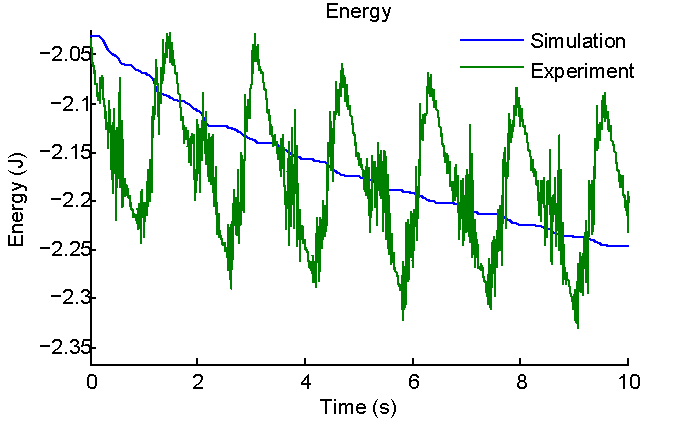
\includegraphics[scale=0.65]{comparison_energy_damped.pdf}
\caption{Comparison of energy over time for simulational and experimental data with damping.}
\label{energyresults}
\end{figure} 

The position and velocity as functions of time for each of the three pendulum links are shown in Figures \ref{positionresults} and \ref{velocityresults} for the tested periodic case.  As shown, the data matches up with the experimental results almost perfectly.

\begin{figure}[H]
\centering
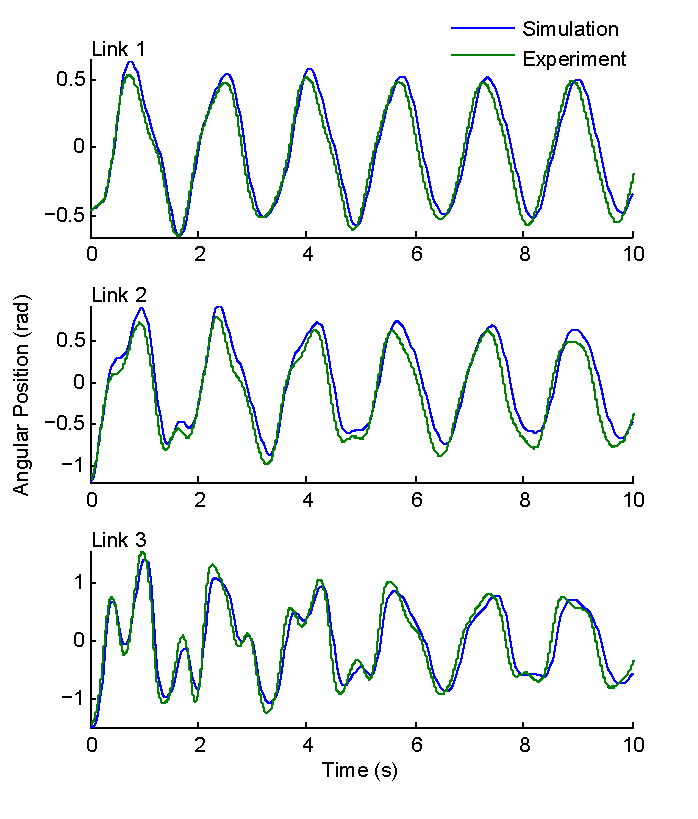
\includegraphics[scale=0.65]{comparison_position_damped.pdf}
\caption{Comparison of position over time for simulational and experimental data with damping.}
\label{positionresults}
\end{figure} 

\begin{figure}[H]
\centering
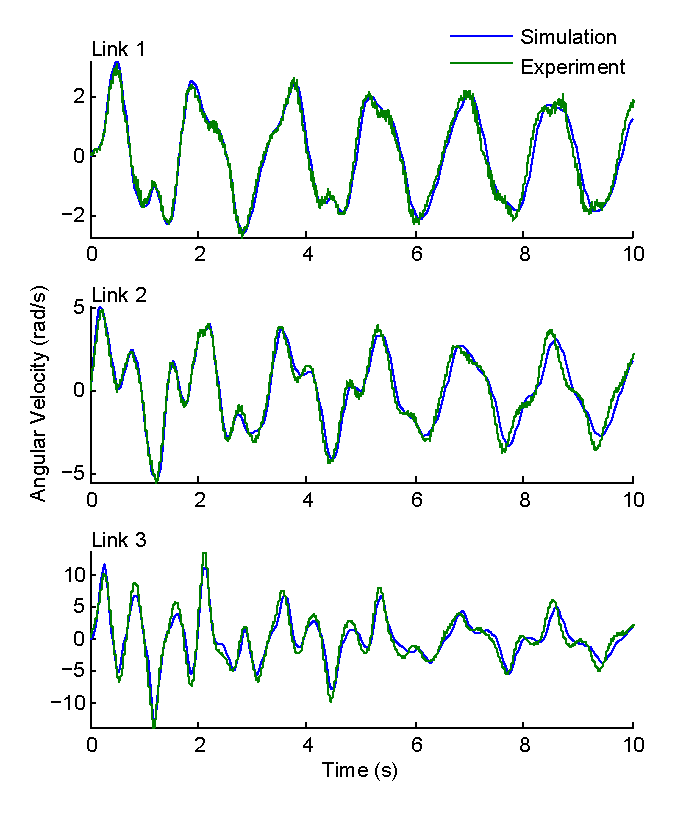
\includegraphics[scale=0.65]{comparison_velocity_damped.pdf}
\caption{Comparison of velocity over time for simulational and experimental data with damping.}
\label{velocityresults}
\end{figure}

When doing the double pendulum, we found that for chaotic systems the modeled and experimental results to separate quickly and postulated that this effect was due to damping in the system which our prior model did not take into account.  This hypothesis was tested by using our simulation to plot the paths of the triple pendulum masses for a set of chaotic initial conditions for both the damped and undamped case (Figure \ref{paths}).  Although there are definite qualitative similarities in the paths of the two masses, the addition of damping causes their paths to differ rather significantly and separate quickly after the first period of high kinetic energy.


\begin{figure}[H]
\centering
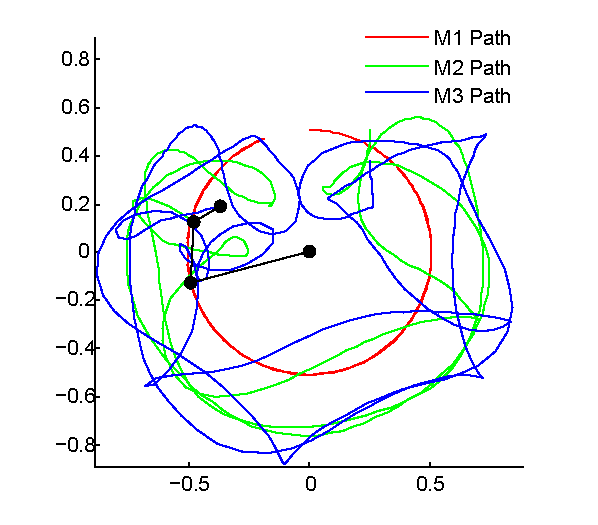
\includegraphics[scale=0.65]{path_nodamping.pdf}
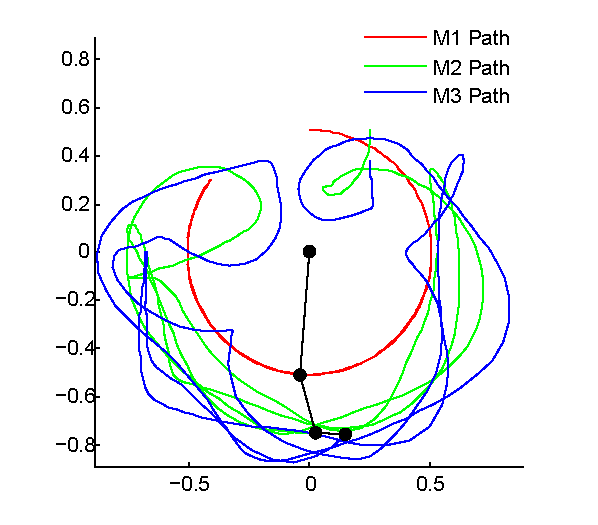
\includegraphics[scale=0.65]{path_damping.pdf}
\caption{The paths of the three links for both (a) undamped and (b) damped cases for a set of chaotic initial conditions.}
\label{paths}
\end{figure}



    \section{Diagnosis}
The largest problems we encountered with this project involved our infamiliarity with Mathematica, the symbolic algebra system we used to solve for the equations of motion. When we started in this project, we knew just enough to get us in trouble. Once we had the Lagrangian, we had difficulty in applying Lagrange's equation to it, as it requires taking derivatives of a function with respect to another function. This combined with our general unfamiliarity with Mathematica syntax made it difficult for us to fix problems. To move forward, we had to step back and go through a few basic Mathematica tutorials. Once we had a stronger grasp on the fundamentals, we found it much easier to solve the problems we were encountering, even though they existed on a higher level of abstraction.

Once we had the equations of motion, we had difficulty in calculating the energies of the system. We had solved the dynamics both using lagrangians and vectors, and our notation did not match between them. Small ambiguities such as the sign of gravity and the definition of our axes were not clearly defined when we began the derivations. This made interpreting the results of the simulation difficult. When we went back to the beginning and explicitly wrote out our system definitions, we were able to more clearly interpret and use our results.

The motion capture system we used to capture experimental data of a real triple pendulum did not tolerate high angular velocities well. It would lose track of links when they began moving too quickly. We could not find an effective fix for this. We made due with what we had by only testing initial conditions which did not produce overly large velocities in the system.

    \section{Improvement}
The main improvements which could be made on the model are for more accurate representations of the damping forces on the system.  This current model takes into effect viscous damping.  A future model could extend this by also including aerodynamic drag as the bars swing through the air.

Furthermore, when testing the system we found that when the pendulum encountered rapid, chaotic movements, the bars of the pendulum encountered dramatic out of plane vibrations.  These vibrations transferred into the table onto which the system was mounted, shaking the table and removing energy from the system.  Although this is a rather complicated damping effect, large quantities of energy were likely lost due to these vibrations and a model of the experimental setup would not be complete without including them.

In addition to adding better models of damping, the model could be made more general by taking it into the third dimension with a three-dimensional triple pendulum.

Finally, there are a number of small physical effects which could be added to the model.  For example, the model could be extended to include the elongation of the steel pendulum rods, the change in gravitational constant as the rods change in elevation or even the gravitational effects of the bars on each other.  However, most of these effects are negligible and would not significantly change the results.

    \section{Reflection}
Leaning about Lagrangian mechanics from an operational perspective was interesting. In some ways it simplifies the derivation of the equations of motion: we had to solve three equations with Lagrangian mechanics instead of the nine we would have needed to do it with Newtonian mechanics. For mechanical systems you are actually trying to design, the Newtonian perspective is vastly better because it gives insight into internal forces which might require structural changes and which variables are most important to the system. We learned that while the Lagrangian method can simplify calculating the dynamics of a system significantly, it is really only useful for a small subset of highly theoretical problems.

Even very small drag forcesmchanged the dynamics of the triple pendulum significantly. This drives home the idea that a triple pendulum is a chaotic system. If small changes in drag create wildly different behaviours you need different techniques to learn someting from your model, because it is unlikely that it will give a highly accurate prediction of the actual behaviour.

We also learned about using Mathematica to do large amounts of simple algebra and calculus. The ability to define intermediate functions allowed us to work on a higher level of abstraction than the gory algebraic details. For example, this allowed us to simple write $v_1$ instead of the long expression corresponding to this in terms of base quantities. This allowed us to see the key components of what we were doing without having to slog through the algebraic detail. However, it was absolutely neccesary to have a strong understanding of what we wanted to do before using Mathematica. This allowed us to better debug the code and interpret its output.

    \section{Conclusion}
Using Lagrangian energy methods, we successfully created a mathematical model featuring a set of coupled ordinary differential equations of motion for the dynamic compound triple pendulum system.  These equations of motion were simulated in MATLAB to create a numerical model of the system.
After tuning damping parameters, the model fit experimental data from the real compound triple pendulum almost perfectly for upwards of ten seconds. 
The behaviour of the model shows that the inclusion of damping forces significantly alters the dynamics of the system after the first few seconds, supporting our hypothesis.  In conclusion, the results of our work supported our hypothesis and we consider this project a success.

    \section{Future Usage}
The step between a double and a triple pendulum is a rather minor one. Mostly it involves more of the same type of mathematics. At most this is character building if solving by hand, but because we used a computer algebra system, it made little difference. It is probably better to instead study a double pendulum. That said, after having done a bob double pendulum, a compound double pendulum, and a triple pendulum, it is interesting to see that the process is really exactly the same. 

However, the introduction of drag into the model was quite interesting. Seeing how this changed the dynamics of the system drove home the chaotic behaviour of the pendulum. Furthermore, thinking about how to represent a drag torque in the mathematical model of the system gave us a greater understanding of what torque is, although this did not make it into the final report.
An appropriate problem state for our project might be:

Consider a planar triple pendulum which consists of three massed bars joined by pivots. The pendulum is fixed to a stable structure at the top bar. Each section has mass $m_1$, $m_2$, and $m_3$ with moments of inertia about the center of mass $I_1$ $I_2$ and $I_3$. 

\begin{itemize}
\item Write the Lagrangian of the system in terms of the angular positions and velocities of the bars.
\item Determine the angular acceleration of the bars with Lagrange's equation.
\item Write a MATLAB script to simulate the motion of the pendulum. Validate your results with a number of initial conditions and show that energy is conserved.
\item Now include damping using Rayleigh's Dissipation Function or some other method. What form of damping would be most accurate? Viscous or aerodyanmic, or something else? What effect does the inclusion of drag have on the dynamics of the system?
\end{itemize}

    
    \begin{thebibliography}{99} % Bibliography - this is intentionally simple in this template
        \bibitem{Widnall}
        Widnall, S. Lecture L20 - Energy Methods: Lagrange’s Equations. N.p.: 16.07 Dyanmics, 2009. PDF. 
        \bibitem{Bann}
        Bannister, Ross. "The Double Pendulum." The Double Pendulum. University of Reading, June 2001. Web. 09 Dec. 2012.
        \bibitem{Von}
        Von Herrath, Franziska, and Scott Mandell. "The Double Pendulum Problem." 19 May 2000. Lecture.
        \bibitem{MT}
        Marion and Thorton, Classical dynamics of particles and systems, 4 ed., Saunders. College Publishing, Fort Worth, TX, 1995.
        \bibitem{Rocky}
        Jones, Rocky M., and Kuch N. Patel. "Examination of Chaos in Multiple Pendulum Systems Through Computer Visualization in Java." Examination of Chaos in Multiple Pendulum Systems Through Computer Visualization in Java. N.p., n.d. Web. 10 Dec. 2012.
    \end{thebibliography}
\end{multicols}

\appendix
    \gdef\thesection{Appendix \Alph{section}}
    \section{Equations of Motion}
\noindent\begin{minipage}{\textwidth}
    \begin{equation}
    \end{equation}
    $\ddot{\theta_1} = -(2 ((l_3^2 m_3^2 \sin(2 \theta_1 - 2 \theta_3) (4 I_2 - l_2^2 m_2) + l_2^2 \sin(2 \theta_1 - 2 \theta_2) (m_2 + 2 m_3) (m_2 m_3 l_3^2 + 4 I_3 (m_2 + 2 m_3))) l_1^2 \dot{\theta_1}^2 + (l_2 (\sin(\theta_1 - \theta_2) ((m_2 m_3 (m_2 + 3 m_3) l_3^2 + 4 I_3 (m_2^2 + 6 m_2 m_3 + 8 m_3^2)) l_2^2 + 4 I_2 (m_3 (m_2 + m_3) l_3^2 + 4 I_3 (m_2 + 2 m_3))) + l_3^2 m_3^2 \sin(\theta_1 + \theta_2 - 2 \theta_3) (4 I_2 - l_2^2 m_2)) \dot{\theta_2}^2 - 4 k_2 l_2 (cos(\theta_1 - \theta_2) (m_3 (m_2 + m_3) l_3^2 + 4 I_3 (m_2 + 2 m_3)) - l_3^2 m_3^2 cos(\theta_1 + \theta_2 - 2 \theta_3)) \dot{\theta_2} + l_3 m_3 (\sin(\theta_1 - \theta_3) (8 I_3 m_3 l_2^2 + 4 I_2 m_3 l_3^2 + 16 I_2 I_3) + l_2^2 \sin(\theta_1 - 2 \theta_2 + \theta_3) (m_2 m_3 l_3^2 + 4 I_3 (m_2 + 2 m_3))) \dot{\theta_3}^2 - 4 k_3 l_3 m_3 (cos(\theta_1 - \theta_3) (2 m_3 l_2^2 + 4 I_2) - l_2^2 cos(\theta_1 - 2 \theta_2 + \theta_3) (m_2 + 2 m_3)) \dot{\theta_3} - g (\sin(\theta_1) ((m_3 (m_1 m_2 + 2 m_1 m_3 + 3 m_2 m_3 + m_2^2) l_3^2 + 4 I_3 (m_2^2 + 6 m_2 m_3 + m_1 m_2 + 4 m_3^2 + 4 m_1 m_3)) l_2^2 + 4 I_2 (m_3 (m_1 + 2 m_2 + m_3) l_3^2 + 4 I_3 (m_1 + 2 m_2 + 2 m_3))) + l_3^2 m_3^2 (\sin(\theta_1 - 2 \theta_3) (4 I_2 - l_2^2 m_2) - 2 l_2^2 cos(2 \theta_2 - 2 \theta_3) \sin(\theta_1) (m_1 + m_2)) + l_2^2 \sin(\theta_1 - 2 \theta_2) (m_2 + 2 m_3) (m_2 m_3 l_3^2 + 4 I_3 (m_2 + 2 m_3)))) l_1 + 2 k_1 (4 I_2 (m_3 l_3^2 + 4 I_3) + l_2^2 (m_3 (m_2 + 2 m_3) l_3^2 + 4 I_3 (m_2 + 4 m_3)) - 2 l_2^2 l_3^2 m_3^2 cos(2 \theta_2 - 2 \theta_3)) \dot{\theta_1}))/(64 I_1 I_2 I_3 + 8 I_3 l_1^2 l_2^2 m_2^2 + 8 I_1 l_2^2 l_3^2 m_3^2 + 8 I_2 l_1^2 l_3^2 m_3^2 + 32 I_3 l_1^2 l_2^2 m_3^2 + 16 I_2 I_3 l_1^2 m_1 + 16 I_1 I_3 l_2^2 m_2 + 64 I_2 I_3 l_1^2 m_2 + 16 I_1 I_2 l_3^2 m_3 + 64 I_1 I_3 l_2^2 m_3 + 64 I_2 I_3 l_1^2 m_3 + 4 I_3 l_1^2 l_2^2 m_1 m_2 + 4 I_2 l_1^2 l_3^2 m_1 m_3 + 16 I_3 l_1^2 l_2^2 m_1 m_3 + 4 I_1 l_2^2 l_3^2 m_2 m_3 + 16 I_2 l_1^2 l_3^2 m_2 m_3 + 48 I_3 l_1^2 l_2^2 m_2 m_3 - 8 I_1 l_2^2 l_3^2 m_3^2 cos(2 \theta_2 - 2 \theta_3) - 2 l_1^2 l_2^2 cos(2 \theta_1 - 2 \theta_2) (m_2 + 2 m_3) (m_2 m_3 l_3^2 + 4 I_3 (m_2 + 2 m_3)) - 2 l_1^2 l_3^2 m_3^2 cos(2 \theta_1 - 2 \theta_3) (- m_2 l_2^2 + 4 I_2) + 2 l_1^2 l_2^2 l_3^2 m_1 m_3^2 + 6 l_1^2 l_2^2 l_3^2 m_2 m_3^2 + 2 l_1^2 l_2^2 l_3^2 m_2^2 m_3 + l_1^2 l_2^2 l_3^2 m_1 m_2 m_3 - 2 l_1^2 l_2^2 l_3^2 m_1 m_3^2 cos(2 \theta_2 - 2 \theta_3) - 4 l_1^2 l_2^2 l_3^2 m_2 m_3^2 cos(2 \theta_2 - 2 \theta_3))$
\end{minipage}

\noindent\begin{minipage}{\textwidth}
    \begin{equation}
    \end{equation}
    $\ddot{\theta_2} = (2 ((l_1^2 \sin(2 \theta_1 - 2 \theta_2) (m_2 + 2 m_3) (m_2 m_3 l_3^2 + 4 I_3 (m_2 + 2 m_3)) - l_3^2 m_3^2 \sin(2 \theta_2 - 2 \theta_3) ((m_1 + 2 m_2) l_1^2 + 4 I_1)) l_2^2 \dot{\theta_2}^2 + l_1 (\sin(\theta_1 - \theta_2) ((m_3 (m_1 (m_2 + m_3) + 2 m_2 (2 m_2 + 3 m_3)) l_3^2 + 4 I_3 (m_2 + 2 m_3) (m_1 + 4 m_2 + 4 m_3)) l_1^2 + 4 I_1 (m_3 (m_2 + m_3) l_3^2 + 4 I_3 (m_2 + 2 m_3))) - l_3^2 m_3^2 \sin(\theta_1 + \theta_2 - 2 \theta_3) ((m_1 + 2 m_2) l_1^2 + 4 I_1)) l_2 \dot{\theta_1}^2 + 4 k_1 l_1 (cos(\theta_1 - \theta_2) (m_3 (m_2 + m_3) l_3^2 + 4 I_3 (m_2 + 2 m_3)) - l_3^2 m_3^2 cos(\theta_1 + \theta_2 - 2 \theta_3)) l_2 \dot{\theta_1} + (- l_3 m_3 (\sin(\theta_2 - \theta_3) ((m_3 (m_1 + 3 m_2) l_3^2 + 4 I_3 (m_1 + 3 m_2 + 2 m_3)) l_1^2 + 4 I_1 (m_3 l_3^2 + 4 I_3)) - l_1^2 \sin(2 \theta_1 - \theta_2 - \theta_3) (m_2 m_3 l_3^2 + 4 I_3 (m_2 + 2 m_3))) \dot{\theta_3}^2 + 4 k_3 l_3 m_3 (cos(\theta_2 - \theta_3) ((m_1 + 3 m_2 + 2 m_3) l_1^2 + 4 I_1) - l_1^2 cos(2 \theta_1 - \theta_2 - \theta_3) (m_2 + 2 m_3)) \dot{\theta_3} + g (\sin(\theta_2) ((m_2 m_3 (2 m_2 + 3 m_3) l_3^2 + 8 I_3 (m_2^2 + 3 m_2 m_3 + 2 m_3^2)) l_1^2 + 4 I_1 (m_3 (m_2 + m_3) l_3^2 + 4 I_3 (m_2 + 2 m_3))) - l_1^2 \sin(2 \theta_1 - \theta_2) (m_3 (m_1 (m_2 + m_3) + m_2 (2 m_2 + 3 m_3)) l_3^2 + 4 I_3 (m_2 + 2 m_3) (m_1 + 2 m_2 + 2 m_3)) + l_3^2 m_3^2 (\sin(\theta_2 - 2 \theta_3) (m_2 l_1^2 + 4 I_1) + l_1^2 \sin(2 \theta_1 + \theta_2 - 2 \theta_3) (m_1 + m_2)))) l_2 - 2 k_2 (4 I_1 (m_3 l_3^2 + 4 I_3) + l_1^2 (m_3 (m_1 + 4 m_2 + 2 m_3) l_3^2 + 4 I_3 (m_1 + 4 m_2 + 4 m_3)) - 2 l_1^2 l_3^2 m_3^2 cos(2 \theta_1 - 2 \theta_3)) \dot{\theta_2}))/(64 I_1 I_2 I_3 + 8 I_3 l_1^2 l_2^2 m_2^2 + 8 I_1 l_2^2 l_3^2 m_3^2 + 8 I_2 l_1^2 l_3^2 m_3^2 + 32 I_3 l_1^2 l_2^2 m_3^2 + 16 I_2 I_3 l_1^2 m_1 + 16 I_1 I_3 l_2^2 m_2 + 64 I_2 I_3 l_1^2 m_2 + 16 I_1 I_2 l_3^2 m_3 + 64 I_1 I_3 l_2^2 m_3 + 64 I_2 I_3 l_1^2 m_3 + 4 I_3 l_1^2 l_2^2 m_1 m_2 + 4 I_2 l_1^2 l_3^2 m_1 m_3 + 16 I_3 l_1^2 l_2^2 m_1 m_3 + 4 I_1 l_2^2 l_3^2 m_2 m_3 + 16 I_2 l_1^2 l_3^2 m_2 m_3 + 48 I_3 l_1^2 l_2^2 m_2 m_3 - 8 I_1 l_2^2 l_3^2 m_3^2 cos(2 \theta_2 - 2 \theta_3) - 2 l_1^2 l_2^2 cos(2 \theta_1 - 2 \theta_2) (m_2 + 2 m_3) (m_2 m_3 l_3^2 + 4 I_3 (m_2 + 2 m_3)) - 2 l_1^2 l_3^2 m_3^2 cos(2 \theta_1 - 2 \theta_3) (- m_2 l_2^2 + 4 I_2) + 2 l_1^2 l_2^2 l_3^2 m_1 m_3^2 + 6 l_1^2 l_2^2 l_3^2 m_2 m_3^2 + 2 l_1^2 l_2^2 l_3^2 m_2^2 m_3 + l_1^2 l_2^2 l_3^2 m_1 m_2 m_3 - 2 l_1^2 l_2^2 l_3^2 m_1 m_3^2 cos(2 \theta_2 - 2 \theta_3) - 4 l_1^2 l_2^2 l_3^2 m_2 m_3^2 cos(2 \theta_2 - 2 \theta_3))$
\end{minipage}

\noindent\begin{minipage}{\textwidth}
    \begin{equation}
    \end{equation}
    $\ddot{\theta_3} = -(2 (32 I_1 I_2 k_3 \dot{\theta_3} - l_2 l_3 m_3 \dot{\theta_2}^2 (\sin(\theta_2 - \theta_3) ((l_2^2 (m_1 m_2 + 4 m_1 m_3 + 6 m_2 m_3 + m_2^2) + 4 I_2 (m_1 + 3 m_2 + 2 m_3)) l_1^2 + 4 I_1 (4 I_2 + l_2^2 (m_2 + 4 m_3))) + l_1^2 \sin(2 \theta_1 - \theta_2 - \theta_3) (m_2 + 2 m_3) (4 I_2 - m_2 l_2^2)) - l_1 l_3 m_3 \dot{\theta_1}^2 (\sin(\theta_1 - \theta_3) (8 I_1 (m_3 l_2^2 + 2 I_2) + 2 l_1^2 ((m_1 m_3 - m_2^2) l_2^2 + 2 I_2 (m_1 + 4 m_2 + 4 m_3))) - l_2^2 \sin(\theta_1 - 2 \theta_2 + \theta_3) (m_2 + 2 m_3) ((m_1 + 2 m_2) l_1^2 + 4 I_1)) + 4 k_3 l_1^2 l_2^2 m_2^2 \dot{\theta_3} + 16 k_3 l_1^2 l_2^2 m_3^2 \dot{\theta_3} + 8 I_2 k_3 l_1^2 m_1 \dot{\theta_3} + 8 I_1 k_3 l_2^2 m_2 \dot{\theta_3} + 32 I_2 k_3 l_1^2 m_2 \dot{\theta_3} + 32 I_1 k_3 l_2^2 m_3 \dot{\theta_3} + 32 I_2 k_3 l_1^2 m_3 \dot{\theta_3} - 4 k_1 l_1 l_3 m_3 \dot{\theta_1} (cos(\theta_1 - \theta_3) (2 m_3 l_2^2 + 4 I_2) - l_2^2 cos(\theta_1 - 2 \theta_2 + \theta_3) (m_2 + 2 m_3)) - 16 I_1 I_2 g l_3 m_3 \sin(\theta_3) - 4 I_2 l_1^2 l_3^2 m_3^2 \dot{\theta_3}^2 \sin(2 \theta_1 - 2 \theta_3) - 4 I_1 l_2^2 l_3^2 m_3^2 \dot{\theta_3}^2 \sin(2 \theta_2 - 2 \theta_3) + 8 I_2 g l_1^2 l_3 m_3^2 \sin(2 \theta_1 - \theta_3) + 8 I_1 g l_2^2 l_3 m_3^2 \sin(2 \theta_2 - \theta_3) + 2 k_3 l_1^2 l_2^2 m_1 m_2 \dot{\theta_3} + 8 k_3 l_1^2 l_2^2 m_1 m_3 \dot{\theta_3} + 24 k_3 l_1^2 l_2^2 m_2 m_3 \dot{\theta_3} - 4 k_2 l_2 l_3 m_3 \dot{\theta_2} (cos(\theta_2 - \theta_3) ((m_1 + 3 m_2 + 2 m_3) l_1^2 + 4 I_1) - l_1^2 cos(2 \theta_1 - \theta_2 - \theta_3) (m_2 + 2 m_3)) - 8 I_1 g l_2^2 l_3 m_3^2 \sin(\theta_3) - 8 I_2 g l_1^2 l_3 m_3^2 \sin(\theta_3) - 4 k_3 l_1^2 l_2^2 m_2^2 \dot{\theta_3} cos(2 \theta_1 - 2 \theta_2) - 16 k_3 l_1^2 l_2^2 m_3^2 \dot{\theta_3} cos(2 \theta_1 - 2 \theta_2) - 8 I_2 g l_1^2 l_3 m_2 m_3 \sin(\theta_3) - 16 k_3 l_1^2 l_2^2 m_2 m_3 \dot{\theta_3} cos(2 \theta_1 - 2 \theta_2) - l_1^2 l_2^2 l_3^2 m_1 m_3^2 \dot{\theta_3}^2 \sin(2 \theta_2 - 2 \theta_3) + l_1^2 l_2^2 l_3^2 m_2 m_3^2 \dot{\theta_3}^2 \sin(2 \theta_1 - 2 \theta_3) - 2 l_1^2 l_2^2 l_3^2 m_2 m_3^2 \dot{\theta_3}^2 \sin(2 \theta_2 - 2 \theta_3) + 2 g l_1^2 l_2^2 l_3 m_1 m_3^2 \sin(2 \theta_1 - \theta_3) - g l_1^2 l_2^2 l_3 m_2^2 m_3 \sin(2 \theta_1 - \theta_3) + 2 g l_1^2 l_2^2 l_3 m_2 m_3^2 \sin(2 \theta_2 - \theta_3) + g l_1^2 l_2^2 l_3 m_2^2 m_3 \sin(2 \theta_2 - \theta_3) + 4 I_2 g l_1^2 l_3 m_1 m_3 \sin(2 \theta_1 - \theta_3) + 8 I_2 g l_1^2 l_3 m_2 m_3 \sin(2 \theta_1 - \theta_3) + 4 I_1 g l_2^2 l_3 m_2 m_3 \sin(2 \theta_2 - \theta_3) - 2 g l_1^2 l_2^2 l_3 m_1 m_3^2 \sin(2 \theta_1 - 2 \theta_2 + \theta_3) - 2 g l_1^2 l_2^2 l_3 m_2 m_3^2 \sin(2 \theta_1 - 2 \theta_2 + \theta_3) - g l_1^2 l_2^2 l_3 m_2^2 m_3 \sin(2 \theta_1 - 2 \theta_2 + \theta_3) + g l_1^2 l_2^2 l_3 m_2^2 m_3 \sin(\theta_3) - g l_1^2 l_2^2 l_3 m_1 m_2 m_3 \sin(2 \theta_1 - 2 \theta_2 + \theta_3)))/(64 I_1 I_2 I_3 + 8 I_3 l_1^2 l_2^2 m_2^2 + 8 I_1 l_2^2 l_3^2 m_3^2 + 8 I_2 l_1^2 l_3^2 m_3^2 + 32 I_3 l_1^2 l_2^2 m_3^2 + 16 I_2 I_3 l_1^2 m_1 + 16 I_1 I_3 l_2^2 m_2 + 64 I_2 I_3 l_1^2 m_2 + 16 I_1 I_2 l_3^2 m_3 + 64 I_1 I_3 l_2^2 m_3 + 64 I_2 I_3 l_1^2 m_3 + 4 I_3 l_1^2 l_2^2 m_1 m_2 + 4 I_2 l_1^2 l_3^2 m_1 m_3 + 16 I_3 l_1^2 l_2^2 m_1 m_3 + 4 I_1 l_2^2 l_3^2 m_2 m_3 + 16 I_2 l_1^2 l_3^2 m_2 m_3 + 48 I_3 l_1^2 l_2^2 m_2 m_3 - 8 I_1 l_2^2 l_3^2 m_3^2 cos(2 \theta_2 - 2 \theta_3) - 2 l_1^2 l_2^2 cos(2 \theta_1 - 2 \theta_2) (m_2 + 2 m_3) (m_2 m_3 l_3^2 + 4 I_3 (m_2 + 2 m_3)) - 2 l_1^2 l_3^2 m_3^2 cos(2 \theta_1 - 2 \theta_3) (4 I_2 - m_2 l_2^2) + 2 l_1^2 l_2^2 l_3^2 m_1 m_3^2 + 6 l_1^2 l_2^2 l_3^2 m_2 m_3^2 + 2 l_1^2 l_2^2 l_3^2 m_2^2 m_3 + l_1^2 l_2^2 l_3^2 m_1 m_2 m_3 - 2 l_1^2 l_2^2 l_3^2 m_1 m_3^2 cos(2 \theta_2 - 2 \theta_3) - 4 l_1^2 l_2^2 l_3^2 m_2 m_3^2 cos(2 \theta_2 - 2 \theta_3))$
\end{minipage}


\end{document}

